\chapter{Cycles as a Graph Invariant}
Cycles is a powerful graph invariant.
In this chapter we will discuss properties of graphs that are reconstructable from Cycles.
We will then show how Cycles is reconstructible from some other graph invariants, which leads us to the conclusion that Cycles is necessarily an incomplete invariant.
We will then discuss manual calculations that find examples of Co-Cycles graphs, and the establishment of small datasets of Co-Cycles graphs as a measure by which to gauge the discriminatory power of graph invariants.
Finally, we will examine the performance of the cycles invariant on different classes of graphs which typically show resistance to classification and differentiation via graph invariants.

\section{Basic Cycles-Reconstructable Properties}

From the Cycles graph invariant, we can easily deduce the number of vertices (the size of the resulting matrix's first dimension), and the number of edges (the sum of the second column of this matrix, divided by two).
We can also deduce the degree sequence, as simply observing the second column of each vertex invariant vector, and sorting the result.

\subsection{Triangles, Higher Order Polygons}
Within the context of a graph, a polygon is similar to a cycle in that both denote closed paths, however, a polygon differs from a cycle in that a cycle is allowed to repeat both edges and vertices, while polygons do not allow repetitions of either (except to close the path to its starting vertex).

The number of triangles is also easily computed.  Since triangles necessarily contain three distinct vertices (in a graph with no self-loops), we know that any cycle of length three on a graph will be a triangle.
Thus, the number of triangles which pass through each vertex is simply the third column of the cycles invariant matrix, and summing them and dividing by three yields the total number of triangles in the graph.

Things are not so simple for larger polygons.  If we think very critically, we can deduce the number of of valid quadrilaterals, by considering the degree sequence of each of the nodes adjacent to a specific node.

Note that this logic requires us to take in an additional piece of information to augment the data that we get from the cycles invariant (i.e. the sum of the degrees of the adjacent nodes).
Similarly, figuring out higher order polygons can be done, but it requires a larger amount of external information.
Generally, the larger the `neighbors-paths' supplemental information we require, the further we stray toward giving away the information that fully determines the graph.

However, this is a powerful observation, and fits into our idea of the cycles invariant as a `neighborhood awareness mechanism'. A formal discussion of such mechanism is discussed in chapter three.

\subsection{Chromatic Polynomial}
One of the most discriminatory polynomial time algorithms for ruling out graph isomorphism is the \emph{Chromatic Polynomial} of the graph's adjacency matrix $A$.
It is a well proven result that shuffling the order of the vertices in the representation of a given graph as an adjacency matrix does not change the eigenvalues of the matrix (thus the eigenvalues, as a multiset, form a powerfully discriminatory graph invariant), and thus the chromatic polynomial (as it encodes all information from this multiset) is also a graph invariant.
In practice, it is a highly discerning as a graph invariant, as a very small proportion of graph instances are ``co-spectral" (having the same chromatic polynomial) and not isomorphic.
However, there are not well established procedures to use the results of eigenvalue calculations to attempt to explicitly construct an isomorphism, rather, it is powerful in ruling out hypothetical isomorphisms.

The large downside of the chromatic polynomial (as a graph invariant) is that it is not computable in polynomial time (across all sets of graphs).
Rather, it is in the computational class $\#P-Hard$ (Sharp-Polynomial Hard), by reducibility to \#3SAT.
There are algorithms which can deterministically solve it in $O(2^N N^r)$ For a constant $r$.
This makes is calculation for graph isomorphism testing prohibitively expensive.
What we will show in this section is objectively quite valuable: we will show that the Cycles invariant encodes the chromatic polynomial, and is actually \emph{more} discriminatory than it.
Thus, by calculating the Cycles invariant, we can discriminate between graphs with greater accuracy, in less time, than by using the chromatic polynomial. 
This result is significant, but requires a long proof.

In seeking out a relationship between the chromatic polynomial and the $Cycles$ invariant, it helps to remember the helpful property of  eigenvalues:
$$E(A) = \{\lambda_1,\lambda_2,\lambda_3, \dots, \lambda_N\} \rightarrow E(A^P) = \{\lambda_1^P,\lambda_2^P,\lambda_3^P, \dots, \lambda_N^P\} $$
Additionally, since we know that our original matrix A is diagonalizable, positive, and symmetric, we know that all of the eigenvalues are real and non-negative. 
Finally, we know that the sum of the diagonal of any matrix is the sum of its eigenvectors. 
Thus, using the $Cycles$ function to determine the entries of the diagonal, we know that for any adjacency matrix A,
$$\lambda_1 + \lambda_2 + \lambda_3 + \dots + \lambda_N = \sum_{i = 0}^{N}{Cycles(A, 1, i)}$$
Or more generally (leveraging our knowledge about the eigenvalues of $A^P$:
$$ \forall_{p \in [1, P]} \; \sum_{i = 0}^N{\lambda_i^p} =  \sum_{i = 0}^{N}{Cycles(A, p, i)}$$
This means that we can create N nonparallel (as not divisible in the ring $R[x]$) equations, each containing $\lambda_1$ to $\lambda_N$ as variables.
Additionally, since we have the guarantee that our eigenvalues are all non-negative, we know that we can assuredly solve any given equation in terms of one of the $\lambda$'s.
If we then use these substitutions, and substitute out all but one of the variables, what we will get is a continuous function whose zeros are well defined and positive. 

Given the aggregated substitution, each one of the zeros is an eigenvalue, assign a selected value to any unassigned eigenvalue, and reduce our equations using that assumed value (think of a let statment).
This kind of procedure is necessary because our system of equations has variables whose relationships are inherently symmetric.
In other words, we cannot make any differentiation between $\lambda_1$ and $\lambda_2$ based on the relationships of the equations, but if we make a choice for either, it will lead to a valid conclusion, or a reduction which does not eliminate a valid conclusion.
This is by virtue of the fact that our substitutions are without condition, and we don't need to worry about any domains of substitution.

From a physical perspective, these equations can be described as surfaces in V dimensions, whose intersection we are interested in isolating for. 
Graphing the equation $x^3 + y^3 + z^3 = \kappa_3$ yields an interesting quasi planar sheet which becomes highly regular at large scales.  
The equation $x^2 + y^2 + z^2 = \kappa_2$ describes a sphere with the radius $\sqrt{\kappa_2}$, and the equation $x + y + z = \kappa_1$ describes a plane. 
Each of these functions is axis symmetric, so their intersections are also axis symmetric.  
The intersection of all of the equations yields a set of points (or none), which represent the potential values for our $\lambda$'s, which are axis invariant. 
We can generalize this to any number of requisite dimensions using the principle of equation and variable symmetry that these equations necessarily produce.

Thus, given the function $Cycles(A, p, v)$, we could calculate the eigenvalues of the matrix A using $Cycles(A, p, v)$ restricted to $1 \leq p \leq P = N$. 
This is superb, as it shows that the $Cycles$ function encodes at least as much information as the chromatic polynomial, and that any graphs which produce the same $Cycles$ function up to (p = V) are co-spectral. 
A quick verification of the base non-isomorphic co-spectral graphs (the butterfly and the box) show that they produce \emph{different} values of the Cycles function, showing that the $Cycles$ function carries \emph{more} information than graph spectrum does, even though both are computed in polynomial time. 
Also helpful: while co-spectral tests might rule out isomorphisms instead of providing a mechanism for their potential generation, the $Cycles$ function suggests the isomorphism that it believes to exist with a natural sorting and comparison of the vectors within the $Cycles$ object.

Again, because of the difference in the running time required to calculate Cycles ($O(N^4)$) versus the running time it takes to calculate the chromatic polynomial ($O(2^N N^r)$), this is an incredibly valuable result: rather than using the chromatic polynomial for discerning between non-isomorphic graphs, it is clear that the Cycles invariant is objectively better.

\subsection{Reconstructing a Valid Graph from Cycles}
If we are given full access to the $Cycles$ function, could we create a graph that is in line with the Cycles invariant?
Note that this question is fundamentally distinct from the one which asks if we could reconstruct the \emph{only} graph that could generate those Cycles values.
That is a separate question, one which the existence of co-cycles graphs makes irrelevant, but the question posed is significantly more general, and does not decide or influence the question of computational complexity of GI.
The reader should note that this section is really a proof of concept and the work done for this was to see how we could go between modes of operation: between reasoning about graphs theoretically, and interacting with them on an algebraic level.
A reader who is focused only on interesting results will not find them in this section.

The answer to this question, fortunately, is yes.  
Over the next few paragraphs, I am going to detail a method of constructing such a graph by first constructing constituent integer-valued equations which describe the interrelationships between edges, then transform the integer edge equations into equally information dense boolean sentences, which by their definition will always hold as true.  
The final step is then to transform each of these sentences into CNF (Codd Normal Form), and use a satisfiability solver to find a solution to them.
[NOTE ON BRUTE FORCE]

Before we begin, lets examine three important points:
\begin{itemize}
  \item{
  	Our reconstruction algorithm is going to run in exponential time, and \emph{that is okay}.  
  	We have already demonstrated that our invariant, the $Cycles$ function, is calculable in polynomial time.  
  	The fact that we can reconstruct a valid graph from the Cycles function is about exploring or debunking the invertible nature of the $Cycles$ object, 
  	and the time it takes to perform an inverse of our operation tells us nothing about the computational complexity of that operation.
  }
  \item{
  	The equations in this section for all but the most trivial of graphs take up an $enormous$ amount of space, and as such, it is not recommended that this reconstruction technique be used in practice.  
  	Realistically, a brute force search would likely yield faster running-solutions (if one were trying to find a graph fitting the Cycles function), but the reader should try to convince themselves that this approach would terminate, 
  	and would yield a valid solution, given a valid $Cycles$ object.
  }
\end{itemize}

We know that the diagonals of $A^p$ yield the $Cycles$ function.
We also know that A is comprised of $(v * (v - 1)) / 2$ boolean variables, and all entries of $A^p$ must be some combination of the variables in the original adjacency matrix. 
We will refer to these variables as the $x_i$'s. Generally, we will arrange them in the row primary pattern, and will number them starting at 1.

The $x_i$'s also have the helpful property that $\forall k \geq 1,\, x_i^k = x_i $. 
This stems from the fact that each one of the $x_i$'s is either zero or one, the two solutions to this identity.  
This allows us to reduce any polynomial degree in our resulting equations down to one, though multivariate linear terms may remain.

I have been discussing these `equations' quite a bit; lets formally define them.  
We assume that we are given the $Cycles$ function for a graph, and we will call $Cycles(p, v) = k_{p, v}$ to simplify our work. 
In each equation, we will set the Cycles function for a specific $v$ and $p$ equal to the symbolic representation of the exponentiated adjacency matrix (which will solely be in terms expressed by the $x_i$'s).
We will refer to this specific equation as Equation p.v for $v$ in the range $[1, V]$ and $p$ in the range $[1, \infty)$.
For each $v$ and $p$ in their respective ranges, our equation p.v is:

$$k_{p, v} = A^p[v,v]$$

Some example Equations are shown below for a five node graph (2.1, 3.1, 4.1). 
Note the rapid expansion in the number and complexity of the terms.  
Also note that we don't need any polynomials over one variable, so we have collapsed them down to their reduced terms.

$$k_{2,1} = x_1 + x_2 + x_3 + x_4$$

$$k_{3,1} = 2x_1x_2x_5 + 2x_1x_3x_6 + 2x_1x_4x_7 + 2x_2x_3x_8 + 2x_2x_4x_9 + 2x_3x_4x_{10}$$

\begin{equation}\begin{aligned} k_{4,1} = x_1 + x_2 + x_3 + x_4 + 2x_1x_2 + 2x_1x_3 + 2x_1x_4 + 2x_2x_3 + x_1x_5 + 2x_2x_4 + x_1x_6 + x_2x_5 \\ + 2x_3x_4 + x_1x_7 + x_3x_6 + x_2x_8 + x_2x_9 + x_3x_8 + x_4x_7 + x_3x_{10} + x_4x_9 + x_4x_{10} \\ + 2x_2x_3x_5x_6 + 2x_1x_2x_6x_8 + 2x_1x_3x_5x_8 + 2x_2x_4x_5x_7 + 2x_1x_2x_7x_9 + 2x_1x_4x_5x_9 \\+ 2x_3x_4x_6x_7 + 2x_1x_3x_7x_{10} + 2x_1x_4x_6x_{10} + 2x_2x_3x_9x_{10} + 2x_2x_4x_8x_{10} + 2x_3x_4x_8x_9 \end{aligned}\end{equation}

An interesting aspect of these equations actually has a cool natural cause.  
Notice that in equation 2.1 and equation 4.1, both have linear terms of four variables.  
(Those happen to be the four variables in the row that we chose, row 1, but if we chose row 4, we would have gotten the variables in that row). 
A nice property that arises out of these linear variables is that if we were to solve for the variable $x_1$ from equation 4.1, we would get an expression with the following denominator: 
$$2x_2 + 2x_3 + 2x_4 + x_5 + x_6 + x_7 + 2x_2x_6x_8 + 2x_3x_5x_8 + 2x_2x_7x_9 + 2x_4x_5x_9 + 2x_3x_7x_{10} + 2x_4x_6x_{10} + 1$$
This is of particular interest, because we know that each one of the terms in this statement has to be positive, as $\forall i \in v,  x_i \in \{0, 1\}$.  
Thus, there is no possible valid input of $x_i$'s which results in this denominator being zero, and our substitution is thus universally valid.  
That is really important because it means that we might be able to do the same thing for other variables, and potentially come up with a system of equations that fully describes the interactions of the vertices within our graph. 
Thus such a system could uniquely determine each of the $x_i$'s, the graph could be determined by $Cycles$, but what what we find instead is that $a$ reconstruction exists, but it is also possible that the reconstruction is not unique.

Lets explore this notion further.  
Lets say that we have an equation that describes the interactions of the binary relations in such a way that we can express the equality for of the variable 
$x_i$ solely in terms of the other variables such that $$x_i = \frac{N}{D + z}$$ Where $z$ is an integer, $z \geq 1$, and $N$ and $D$ 
can be any number of positive expressions that are comprised of terms of the addition and multiplication of variables in the set 
$\{x_1, \dots,  x_{i-1},x_{i+1}, \dots, x_{(v(v-1))/2}\}$.  Since we know that $x_i \in {0,1}$, we know that any positive term comprised of the multiplication and addition of these variables must be greater than or equal to zero.  
Thus, we know the denominator of the equation for $x_i$ must be greater than or equal to one ($D + z \geq 1$). 
This is a helpful result, as it means that our substitution is valid, and we know that the equality holds, because our division of both sides by $D + z$ 
does not risk dividing by zero.  We will call this a \emph{valid substitution} for $x_i$ over the equation for which it is generated (e.g. Equation 2.5). 

It turns out that there is a clever way to use a \emph{valid substitution} to construct a graph which would generate the Cycles functions that generated the equations which generated the valid substitutions.
Since we know that the denominator of a valid substitution is non-zero, we know the substitution is valid.  
We also happen to know that the variable we are solving for is either equal to zero or one.  
Thus, if the numerator ($N$) of our substitution is equal to zero, then we know that $x_i$ is equal to zero.  
Otherwise, we know that $x_i$ must be equal to one (for all other values are not in its domain). 
If we allow ourselves to do an informal conversion to predicate logic, we can transform an equation of the form:
 $$x_i = \frac{N}{D + z}$$ 
 $$(x_i = 0) \; \text{iff} \; (N = 0)$$
 $$\neg(x_i) \; \text{iff} \; (N = 0)$$
 $$x_i  \leftrightarrow  \neg(N = 0)$$
Expressing that $N$, a summation of terms over the $x_i$'s, is equal to zero, is actually quite a simple construct. 
We imagine that each of the terms in N has a positive, integer valued weight that corresponds to its coefficient. 
If $N$ contains any integer valued negatives (which it does in real applications), we will call this the $target$.
Given this (and the terms and their weights as corresponding lists), we can generate a simple procedure for generating a boolean statement that encodes the information that our equation does when $N$ is set to zero.

\begin{lstlisting}[frame=single]
exactlyKTrue(clauses, weights, target):
	if (target == 0) then
		return negatedConjuction(clauses)
	clause = clauses.pop()
	weight = weights.pop()
	caseF = exactlyKTrue(clauses, weights, target)
	newTarget = target - weight
	caseT = exactlyKTrue(clauses, weights, newTarget)
	return (clause & caseT) | (!clause & caseF))
\end{lstlisting}

Though this code doesn't totally cover all edge cases, it should convince the reader that there is an appropriate transform between $N$ and a boolean expression of the $x_i$'s which maintains domain validity across substitutions.

\section{Other Forms of Reconstructability}
\subsection{EA Reconstructability}
\subsection{Deck Reconstructability}

\section{Placing Cycles within a Time/Power Tradeoff}
A subjective task we have to undertake is the critical examination of Cycles within the invariant tradeoff between computational power and time complexity.
On the one hand, cycles is highly discriminatory, and for the majority of graphs, we can show that cycles distinguishes between vertices in a way which fully distinguishes them.
This computational power means that for the overwhelming majority of graphs (particularly large graphs), cycles can give us canonical labelings with a single pass.

However, on the other hand, cycles is heavy handed. There is a constant amount of work that has to be done to calculate cycles for any number of vertices in the graph. 
This means that even if we had a graph where every node was distinguished only by its degree, we would still require an extensive process of matrix multiplication to even get to results that could have been achieved in less time by any other means.

One way we can discuss this tradeoff is computationally.
An invariant that is `good' distinguishes between non-similar vertices in a small amount of time.
An invariant is `worse' the more time it takes to compute.

[COMPUTATIONAL RESULTS HERE] 

%\section{Discrimination on Tough Graph Classes}
%\subsection{Background}
%Any algorithm or methodology we create needs to be verified in the same terms that precursors have used to verify themselves.
%One way to do this is to examine the performance of tasks (such as canonical labeling and isomorphism testing) on the same classes of graphs that established renditions of those algorithms have used to push their performance.
%The most established canonical labeler comes from the NAUTY package CITE.
%The three sets of graphs that the authors of that package use to push the performance of their algorithm are the 1-Sparse, 2-Dense, and Miyizaki Graphs, each of which present their own set of challenges.
%In this section, we will briefly outline each of these sets of graphs, then show how a cannonical labeler based in cycles performs on each, comparing against NAUTY benchmarks.
%
%\subsection{1-Sparse Graphs}
%
%\subsection{2-Dense Graphs}
%
%\subsection{Miyizaki Graphs}

\section{Discrimination on Tough Graph Classes}

\subsection{Miyizaki Graphs}
The Miyizaki Graphs are as interesting as they are inscrutable.
They were described in a paper by CITE in CITE, and can be summarized as being comprised of similar constructions that are occasionally twisted.
It does not come as a surprise to me, and it should not come as a surprise to you, that the cycles invariant is unable to distinguish in between any Mikizaki Isomorphism pairs.

Miyizaki graphs are co-cycles graphs in partnership with their twisted halves.
In testing this hypothesis, I tested it on the Miyizaki graphs:
\begin{itemize}
\item{TODO}
\end{itemize}
and each were shown to be co-cycles.

However, differentiation with flagging (as described in the chapter on vertex invariants) was possible, at enormous computational (though still polynomial!) expense.

\section{Imperfection, Co-Cycles Graphs}

Though it has been alluded to previously, a key discovery of my thesis is that there exist co-cycles graphs, non-isomorphic graphs which have the same value for the cycles invariant for all observed values of P.
These graphs are incredibly rare.
None exist with fewer than ten vertices, and only about 100 of the 12 million graphs over 10 vertices satisfy this property.

In this section, we will discuss the initial discovery of co-cycles graphs, detailing the relatively advanced set of methodologies used.
Then we will discuss how co-cycles graphs can be constructed intentionally, on larger sets of vertices.
Finally, we will discuss co-cycles graphs as a useful (and relatively small) set of graphs which are useful for invariant analysis and testing.

\subsection{Discovering Co-Cycles Graphs, Cleverly}

Discovering co-cycles graphs was not trivial.
The way I went about looking for them was theoretically simple, but incredibly challenging to implement and process.
\begin{itemize}
\item{First, I enumerated all graphs of size N with M vertices by using the NAUTY geng function}
\item{I set up a mechanism which delivered the cycles values in sorted order, thus, the cycles invariant (which is an $N \times N$ matrix) could be parsed apart in order of its columns (all of the values of cycles of length 2, then 3, then 4, etc)}
\item{I used a clever set of minimally memory intensive structures to store only the information needed for a given unit of this computation.  This, in combination with the second step, yielded a delayed stream processing, where we have a structure (with minimal memory), which can be called upon for another, more differentiating value.}
\item{These structures (one per graph), were placed in an enormous trie, each level of which was the level of the delayed evaluation.  Only values which differentiated between different structures were evaluated (lazy eval on trie-collision, splitting into sub-tries).}
\item{Co-Cycles graphs were then simply detected by depth. After all graphs of a given size (with a given number of edges) were placed into the trie, only those at depth $N^2$ could possibly be co-cycles.}
\end{itemize}

The lazy evaluation (in a couple of benchmark tests on eight vertices) worked more efficiently on the order of $10^{-3}$ times the original running time.
Additionally, a trick I employed with bulk memory allocation reduced running time on the order of $10^-1$ (allocated 100 trie-nodes at once, rather than 1 at a time).
An additional optimization I made was the singular evaluation of a combination of N and M at a given time.
We know that the number of vertices and edges in a graph is reconstructible from the cycles invariant, so we only need to check for set values of M and N if we want to discover co-cycles graphs.
This enabled me to reduce the overall amount of memory allocated to approximately a tenth of what it would require to process all graphs of a given size simultaneously.

Additionally, a smart way that I set up my matrices allowed for insanely efficient memory allocation: since I had to maintain every single graph in my trie, for even a small number of vertices that could have been an incredible amount of space.
The graphs themselves were stored as pointers to arrays of integers (int**), which leads to a costly price in memory for even a small N (consider N=10):
$$Memory Used = SizeOf(Int) * N * N * NGraphs + SizeOf(Int*) * N * NGraphs = 4 * 10 * (10+2) * 12,005,168 = 5,762,480,640 \approx 6 GB $$
However, I realized quite quickly that since the matries themselves were not chaning over the course of the computation (the were being used in mutliplcations and what not, and being used to change other values and matrices), we could share their representations.
I decided not to have my algorithm waste time trying to canonize the graphs or find similarities, or shrinking down the individual memory storage of the graphs to the bit level (which would have been highly inefficient for the frequent scale-up/down necessary for computations as integers).
Instead, I simply pre-allocated all of the $2^N$ possible vectors that could be sub-vectors of a matrix.
Thus, the only thing that changed was that each of the individual entries in this great large computation is pre-allocated and shared amoungst all 12 million graph representations as in $N = 10$.  The memory use for this case is shown to be dramatically reduced:
$$Memory Used = SizeOf(Int) * N * NVectors + Sizeof(Int*) * N * NGraphs = 4 * 10 * 2^{10} + 8 * 10 * 12,005,168 = 960,454,400 \approx 1 GB $$



\subsection{Constructing Co-Cycles Graphs}
\subsection{As a Proposed Dataset for Invariant Analysis}

\section{Trie Depth and the Power of Cycles Across Classes of Graphs}

In chapter three, we will discuss a notion of $P^*(G)$, a value for which (within a graph G), cycles beyond length $P^*(G)$ do not yield additional discriminatory information.
Related is the same idea across sets of graphs.
For example, if we have some set of graphs $S$, there exists an integer $P^*(S)$, at which values beyond this length cycle are not informative in further discriminating between graphs in the set.
Intuitively, for a set with one element, $P^*(S) = 0$, and not-so-intuitively, with a set with only graphs which are co-cycles with one another, $P^*(S) = 0$.

The way that  $P^*(S)$ is calculated takes a natural interpretation within our co-cycles computations in C. 
 $P^*(S)$ is simply the maximum depth of the trie created when searching for co-cycles graphs, excepting nodes of full ($N^2$) depth.

\subsection{Expectations Borne out of Graph Counts}

A natural cadre of sets to explore is $S_{N, M} = Graphs(N, M)$, where $S_{N, M}$ is the set of all graphs with $N$ vertices and $M$ edges.
Before we discuss the results of what we observed $P^*(S)$ to be over these sets, lets first discuss what we anticipate, and discuss a detail of its implementation.
Naturally, we would think that the larger the set $S$, the more difficult it will be to fully discriminate between all of the graphs in it.
If we fix N, the distribution of graphs within that N over various values of M is approximately normal, and approximation that increases in accuracy as N increases (see chapter 1).
Thus, if we intuit that $P^*(S)$ is likely to be a function of the size of S, we would expect $P^*(S)$ to be approximately normally distributed.

What we actually find is markedly different, in the next three diagrams, of this curve for N=8, 9 and 10:

\begin{figure}[h]
\label{fig:powercurve8}
\caption{}
\centering
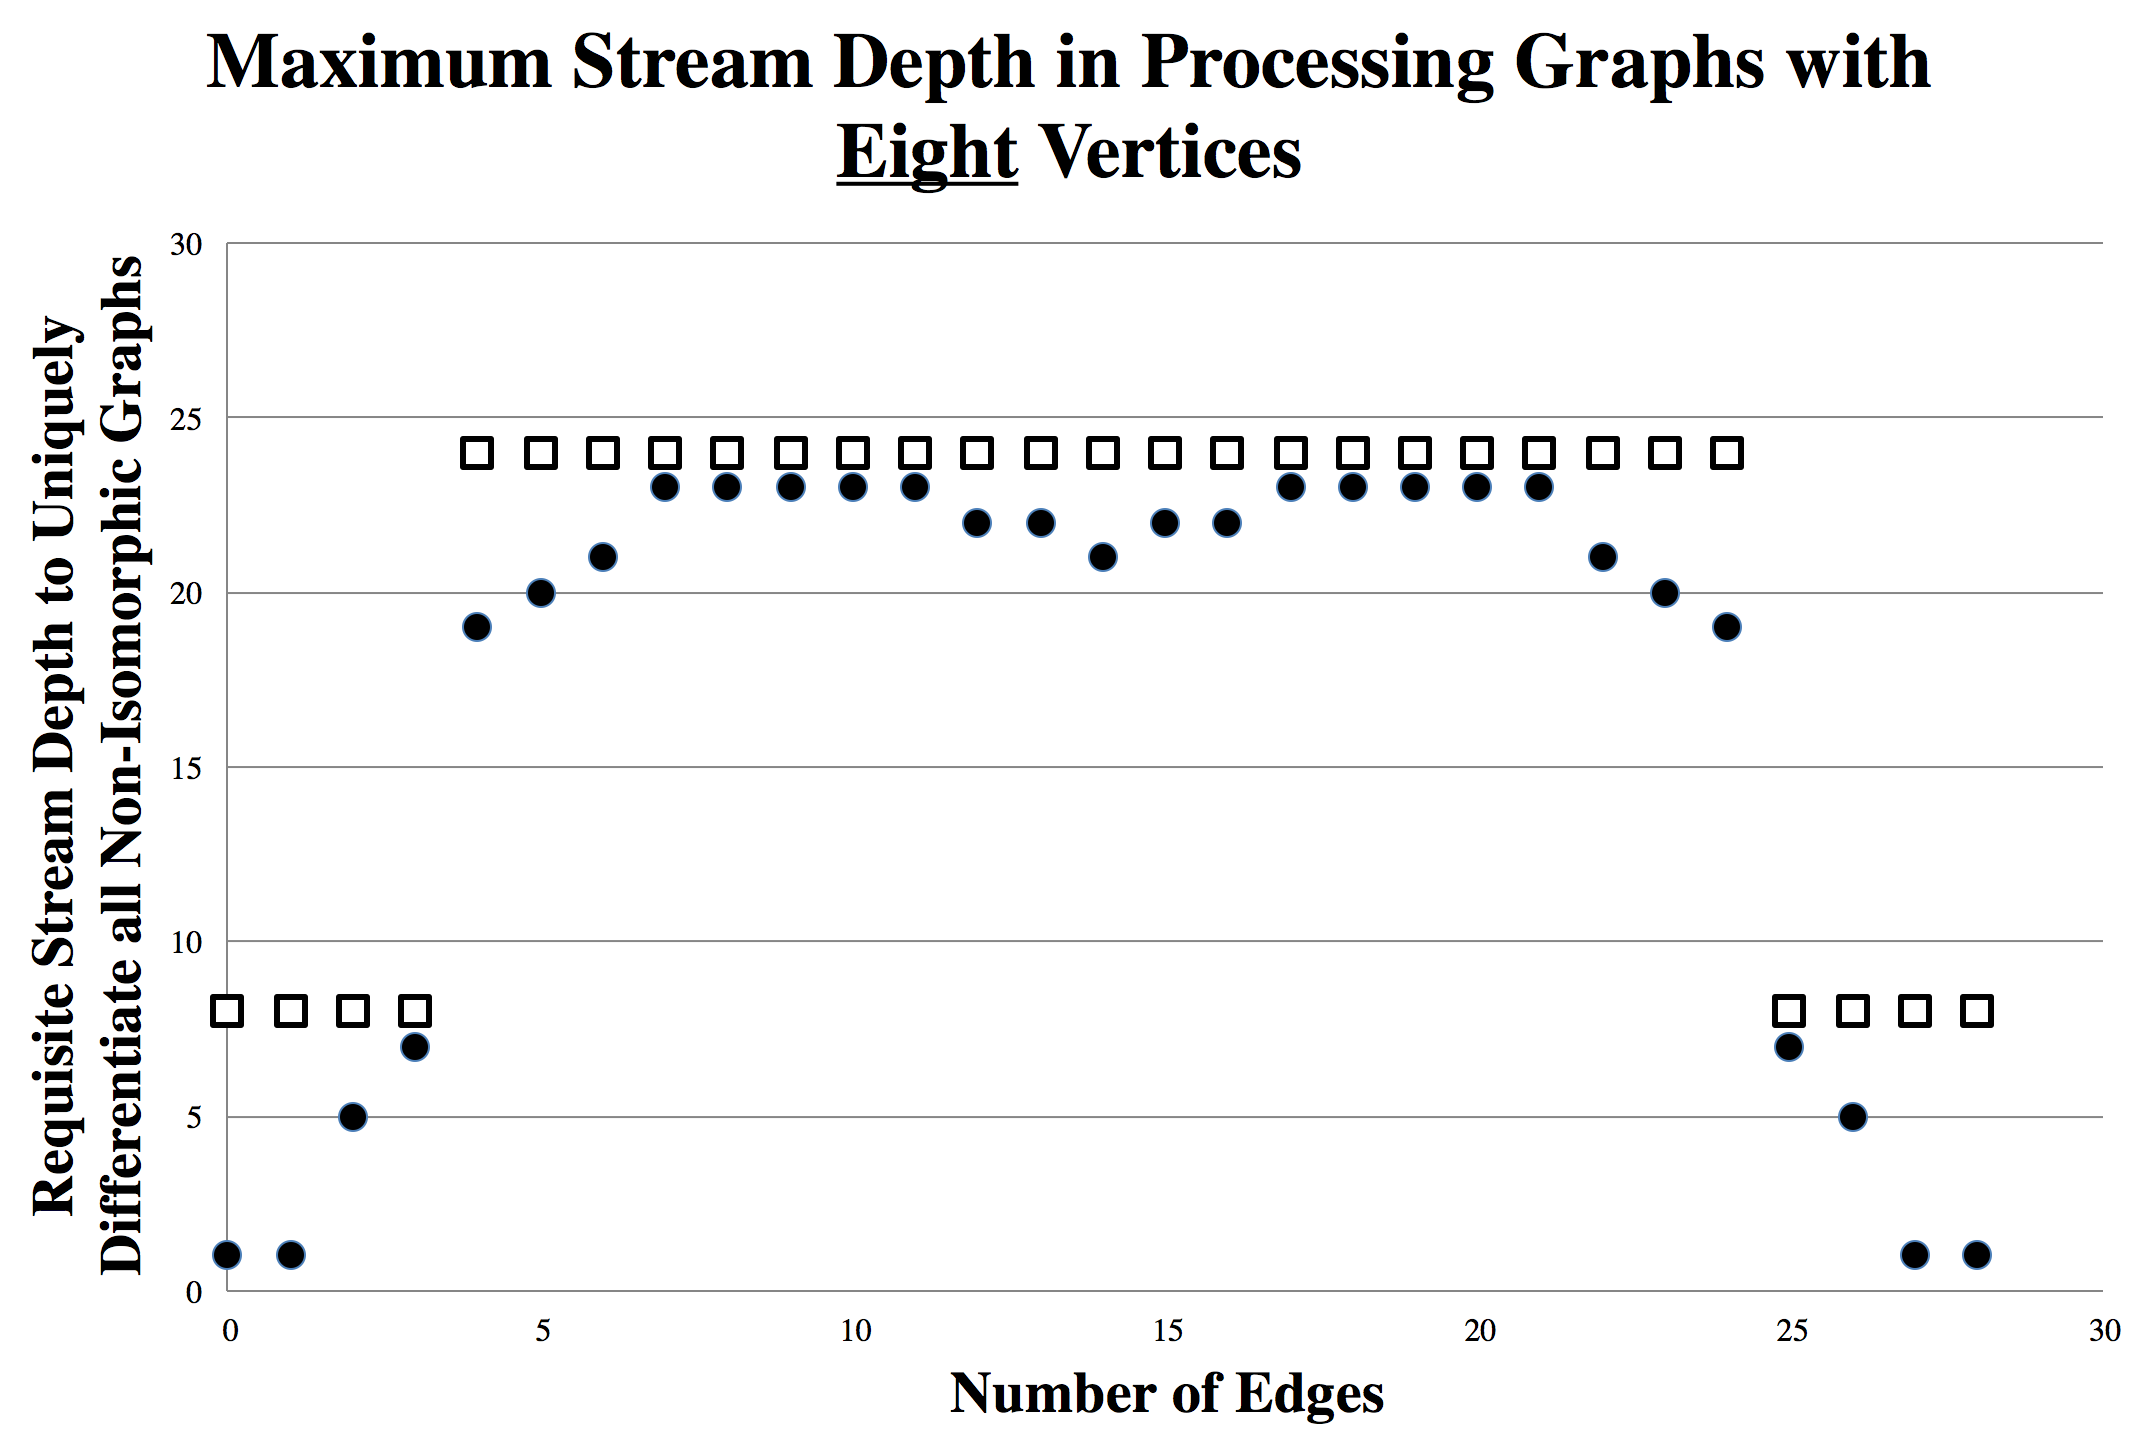
\includegraphics[width=\textwidth]{powercurve8}
\end{figure}

\begin{figure}[h]
\label{fig:powercurve9}
\caption{}
\centering
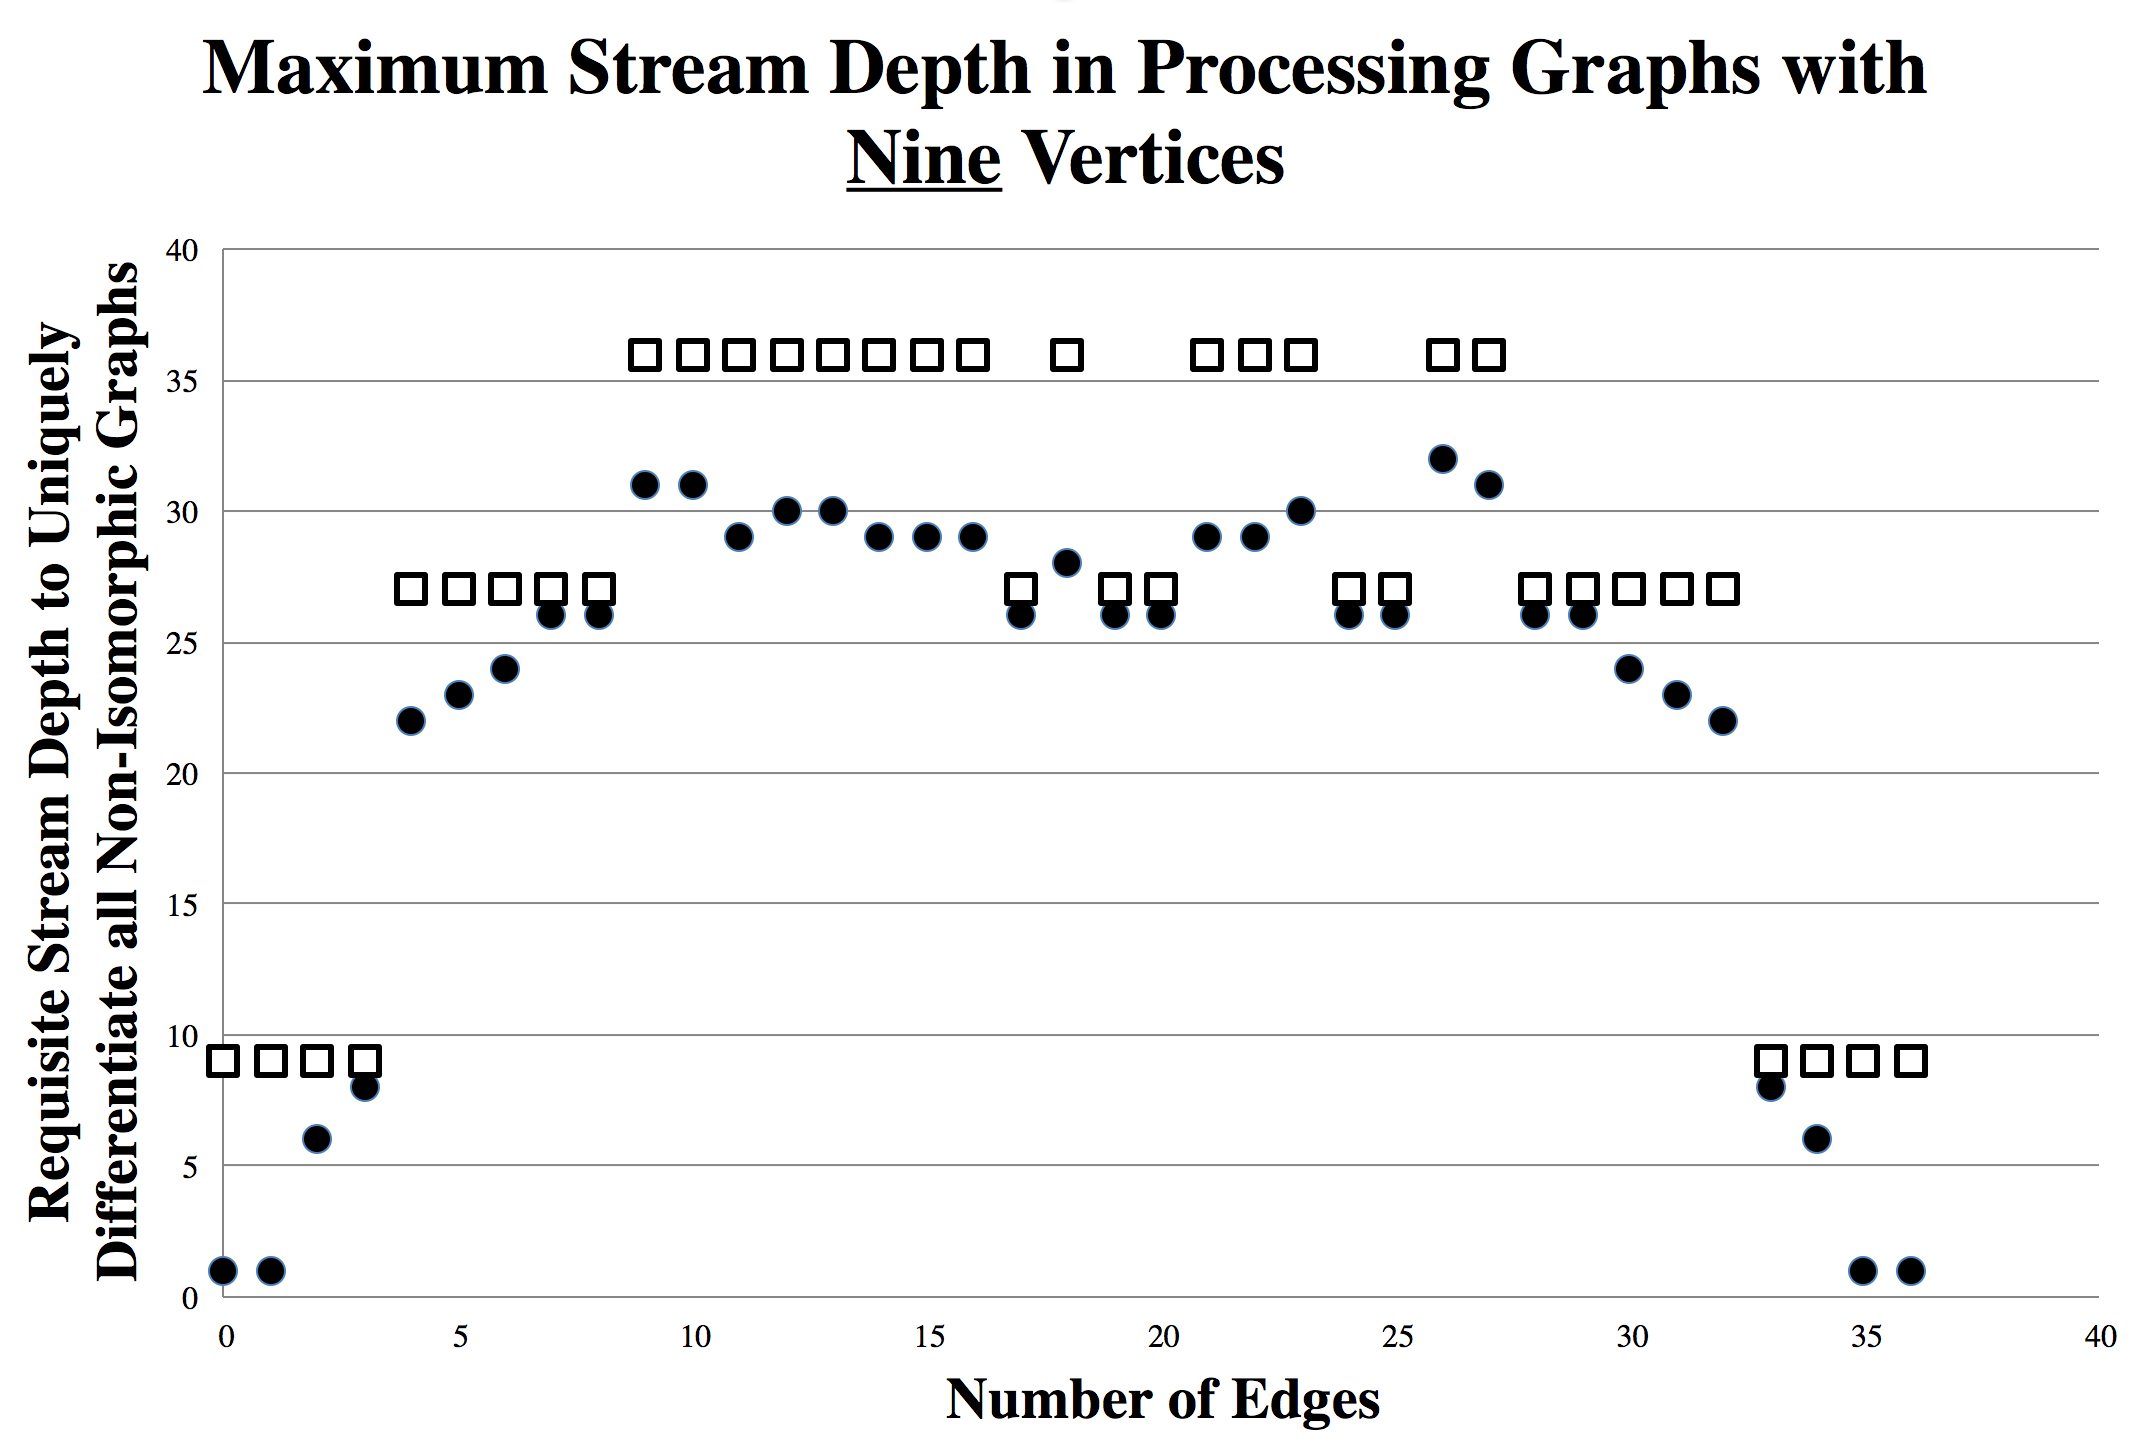
\includegraphics[width=\textwidth]{powercurve9}
\end{figure}

\begin{figure}[h]
\label{fig:powercurve10}
\caption{}
\centering
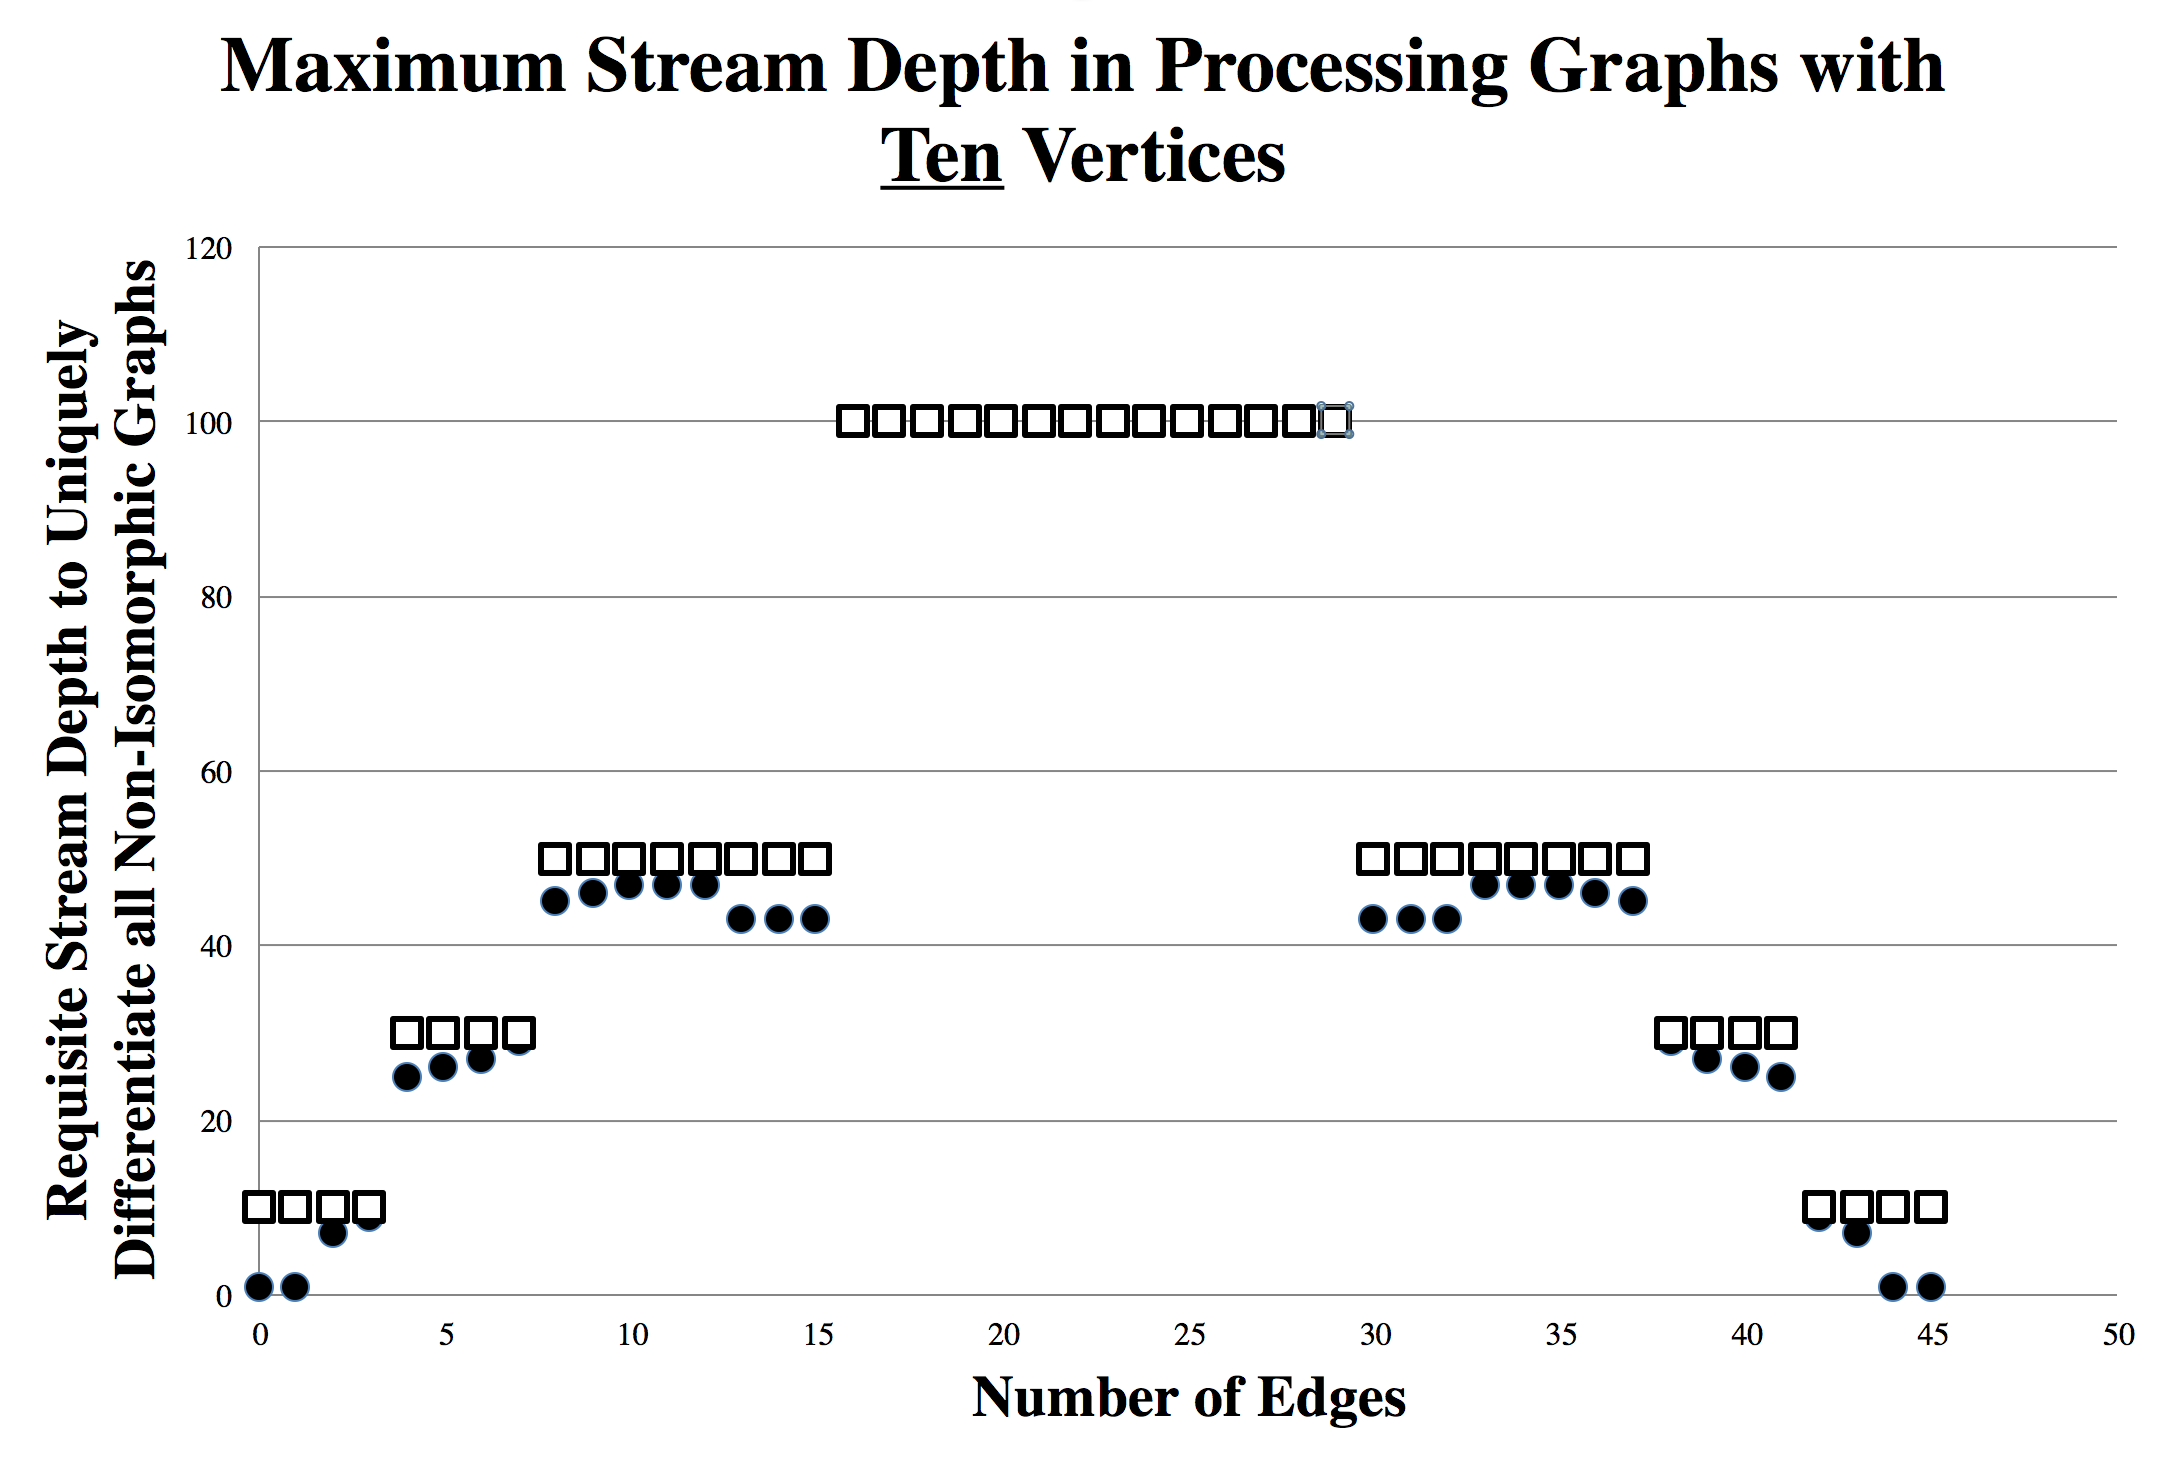
\includegraphics[width=\textwidth]{powercurve10}
\end{figure}

In each diagram, the dots represent the maximum trie depth, while the squares above them round that value up to the nearest `complete' depth.
By complete depth, we are referring to a depth divisible by the number of vertices within the graph.
This is relevant because these levels are the length of the cycles that correspond to all of the information gleaned from this length cycle and fewer.

\subsection{An Unexpected Dip}

What we see is counter to our expectations.
$P^*(S_{N, M})$ certainly is smaller at the fringes, but it actually dips in the middle, where the majority of the graphs are located.
Remember from chapter one that the number of graphs in each of these sets is maximized in the middle, while the ability to differentiate between them is actually maximized with connectivity around .25 and .75.

In figure \ref{powercurve10}, we see the same trend (slightly lower values for $N > 12$, than for $N \in (10, 12)$), despite the existence of co-cycles graphs, which push the middle up to 100 (maximal trie depth for N=10).

In figure \ref{powercurve9}, we see this trend exaggerated to the point that it distorts not only the granular values (the black dots), but the overall cycles length values (boxes).

It should be noted that the asymmetry in diagram \cite{powercurve9} was highly suspect to me.
I looked into it, and was able reproduce it using Matlab (in addition to the calculations in C).  
It turns out that the asymmetry is due to the lack of invertible equivalence in the Cycles invariant, and for some graphs in $S_{N=9, M=25}$ can be differentiated by their cycles values, while their inverses cannot.

This small set of experiments suggests an interesting property of graphs: it may be easier to differentiate between graphs which are half connected than a quarter connected, despite the fact that there are significantly more graphs which are half connected.
